\documentclass[11pt]{article}
\usepackage[utf8]{inputenc}
\usepackage{centernot}
\usepackage[parfill]{parskip}
\usepackage{amsmath}
\usepackage{amssymb}
\usepackage{graphicx}
\begin{document}
\title{Algebra Problem 5}
\author{Robin Boregrim}
\maketitle
\renewcommand{\contentsname}{Innehållsförteckning}
\tableofcontents
\newpage
\section{Uppgiften}
Låt $A$, $B$, $C$ och $D$ utgöra hörnen på en fyrhörning i planet. Vektorerna $e_1 = \overline{AB}$ och $e_2 = \overline{AC}$ utgör en bas för planet och vektorerna $f_1 = \overline{AD}$ och $f_2 = \overline{BC}$ utgör en annan bas. Antag att fyrhörningen är sådan att $\overline{AD} = \frac{2}{3}\overline{AB} + \frac{3}{4}\overline{AC}$. Uttryck vektorerna $e_1$ och $e_2$ i vektorerna $f_1$ och $f_2$.
\section{Lösning}
För att lättare kunna se samband så börjar vi med att göra en skiss av problemet.
$$
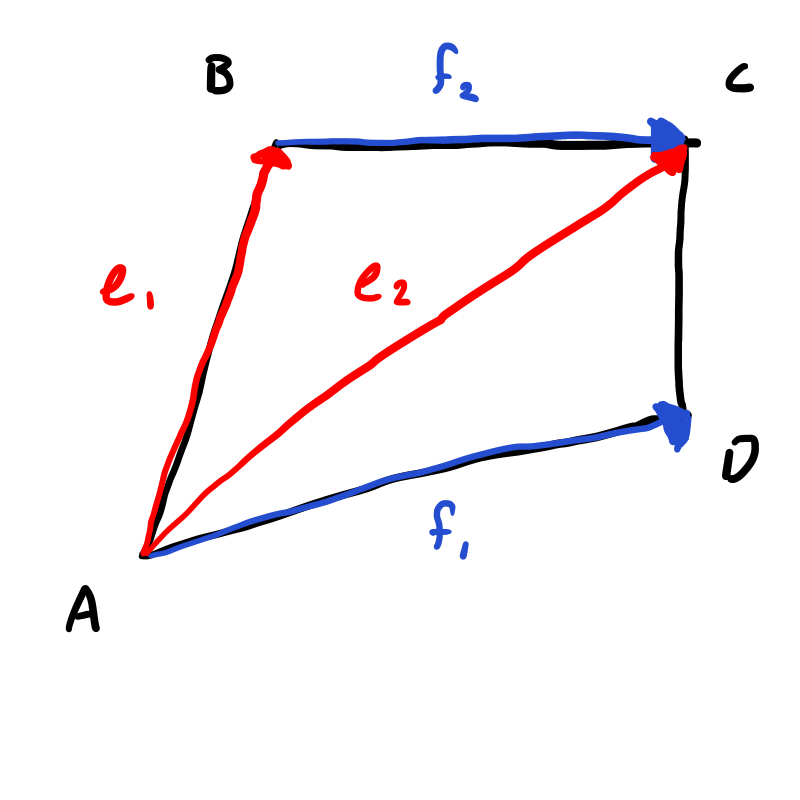
\includegraphics[scale=1]{figure1}
$$
Vi vet:
$$
\left\{\begin{array}{c}
e_1 = \overline{AB}\\
e_2 = \overline{AC}\\
f_1 = \overline{AD} \\
f_2 = \overline{BC}\\
\overline{AD} = \frac{2}{3}\overline{AB} + \frac{3}{4}\overline{AC}
\end{array}\right.
$$
Vi kan skriva om
$$\overline{AD} = \frac{2}{3}\overline{AB} + \frac{3}{4}\overline{AC}  \Rightarrow$$ till
\begin{equation}\label{1}
	f_1 = \frac{2}{3}e_1 + \frac{3}{4}e_2
\end{equation}
Och ifrån skissen kan vi läsa av att 
\begin{equation}\label{2}
	e_1 = e_2 - f_2
\end{equation}
Vi stoppar in uttrycket för $e_1$ från (\ref{2}) i (\ref{1}) och förenklar.
$$f_1 = \frac{2}{3}(e_2 - f_2) + \frac{3}{4}e_2$$
$$f_1 = \frac{2}{3}e_2 + \frac{3}{4}e_2 - \frac{2}{3}f_2 $$
$$f_1  = \frac{8+9}{12}e_2 -\frac{2}{3}f_2$$
$$\frac{17}{12}e_2= f_1 + \frac{2}{3}f_2$$
$$e_2=\frac{12}{17} (f_1 + \frac{2}{3}f_2)$$
\begin{equation}\label{3}
e_2=\frac{12}{17}f_1 + \frac{8}{17}f_2
\end{equation}
Vi stoppar sedan in värdet på $e_2$ från(\ref{3}) i (\ref{2}).
$$e_1 = (\frac{12}{17}f_1 + \frac{8}{17}f_2) - f_2 $$
$$e_1 = \frac{12}{17}f_1 - \frac{9}{17}f_2$$
Och då har vi uttryckt vektorerna $e_1$ och $e_2$ med vektorerna $f_1$ och $f_2$.
\subsection{Svar}
Vi kan skriva $e_1$ och $e_2$ som:
$$e_1 = \frac{12}{17}f_1 - \frac{9}{17}f_2$$
$$e_2=\frac{12}{17}f_1 + \frac{8}{17}f_2.$$
\end{document}